\documentclass[12pt]{article}
\setlength{\oddsidemargin}{0in}
\setlength{\evensidemargin}{0in}
\setlength{\textwidth}{6.5in}
\setlength{\parindent}{0in}
\setlength{\parskip}{\baselineskip}
\usepackage{amsmath,amsfonts,amssymb}
\usepackage{graphicx}
\usepackage{enumitem}
\usepackage[]{algorithmicx}
\usepackage{amsthm}
\usepackage{fancyhdr}
\pagestyle{fancy}
\setlength{\headsep}{36pt}
\usepackage{tkz-berge}
\usetikzlibrary{positioning, automata}

\usepackage{hyperref}

\theoremstyle{remark}
\newtheorem*{solution}{Solution}

\newcommand{\makenonemptybox}[2]{%
%\par\nobreak\vspace{\ht\strutbox}\noindent
\item[]
\fbox{% added -2\fboxrule to specified width to avoid overfull hboxes
% and removed the -2\fboxsep from height specification (image not updated)
% because in MWE 2cm is should be height of contents excluding sep and frame
\parbox[c][#1][t]{\dimexpr\linewidth-2\fboxsep-2\fboxrule}{
  \hrule width \hsize height 0pt
  #2
 }%
}%
\par\vspace{\ht\strutbox}
}
\makeatother

\begin{document}

\lhead{{\bf CSCI 3104, Algorithms \\ Problem Set 9a (7 + 5 extra credit = 12 points)} }
\rhead{Name: \fbox{Michael Rogers} \\ ID: \fbox{105667404} \\ {\bf Profs.\ Hoenigman \& Agrawal\\ Fall 2019, CU-Boulder}}
\renewcommand{\headrulewidth}{0.5pt}

\phantom{Test}

\begin{small}
\textit{Advice 1}:\ For every problem in this class, you must justify your answer:\ show how you arrived at it and why it is correct. If there are assumptions you need to make along the way, state those clearly.
\vspace{-3mm} 

\textit{Advice 2}:\ Verbal reasoning is typically insufficient for full credit. Instead, write a logical argument, in the style of a mathematical proof.\\
\vspace{-3mm} 

\textbf{Instructions for submitting your solution}:
\vspace{-5mm} 

\begin{itemize}
	\item The solutions \textbf{should be typed} and we cannot accept hand-written solutions. \href{http://ece.uprm.edu/~caceros/latex/introduction.pdf}{Here's a short intro to Latex.}
	\item You should submit your work through \href{https://www.gradescope.com/courses/59294}{\textbf{Gradescope}} only.
	\item If you don't have an account on it, sign up for one using your CU email. You should have gotten an email to sign up. If your name based CU email doesn't work, try the identikey@colorado.edu version. 
	\item Gradescope will only accept \textbf{.pdf} files (except for code files that should be submitted separately on Gradescope if a problem set has them) and \textbf{try to fit your work in the box provided}. 
	\item You cannot submit a pdf which has less pages than what we provided you as Gradescope won't allow it. 
\end{itemize}
\vspace{-4mm} 
\end{small}

\hrulefill
\pagebreak


\begin{enumerate}

\item (7 pts) Consider the following DP table for the Knapsack problem for the list $A = [(4, 3), (1, 2), (3, 1), (5, 4), (6, 3)] $ of (weight, value) pairs. The weight threshold $W = 10$.
\begin{itemize}
    \item Fill in the values of the table.
    \item Draw the backward path consisting of backward edges and do not draw (or erase them) the edges that are not part of the optimal backward paths.
\end{itemize}

\begin{enumerate}
    \item (4 pts) Fill the table with the above requirements (You can also re-create this table in excel/sheet).
    \begin{solution}

    \end{solution}


\begin{figure}[h!]
\begin{center}
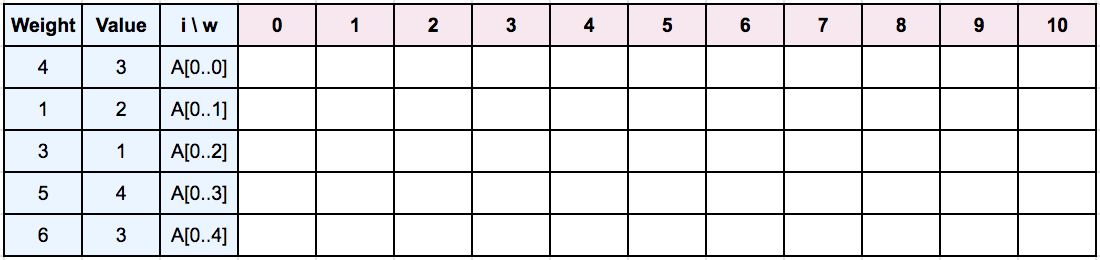
\includegraphics[scale=0.9]{DP_PS9a.png}
\end{center}
\end{figure}
    \item (1 pts) Which cell has the optimal value and what is the optimal value for the given problem?
    \begin{solution}

    \end{solution}
    
    \item (2 pts) List out the optimal subset and provide it's weight and value.
    \begin{solution}

    \end{solution}

\end{enumerate}
\pagebreak
    
        \item (5 pts) [\textbf{Extra Credit}] Given the following directed acyclic graph, and assume a ``path'' must have at least one edge in it to be well defined. Use dynamic programming to fill in a table that counts number of paths from each node $j$ to 14, for $j \geq 1$. 

        % ----- FIGURE -----
        \begin{figure}[h!]
        \begin{center}
        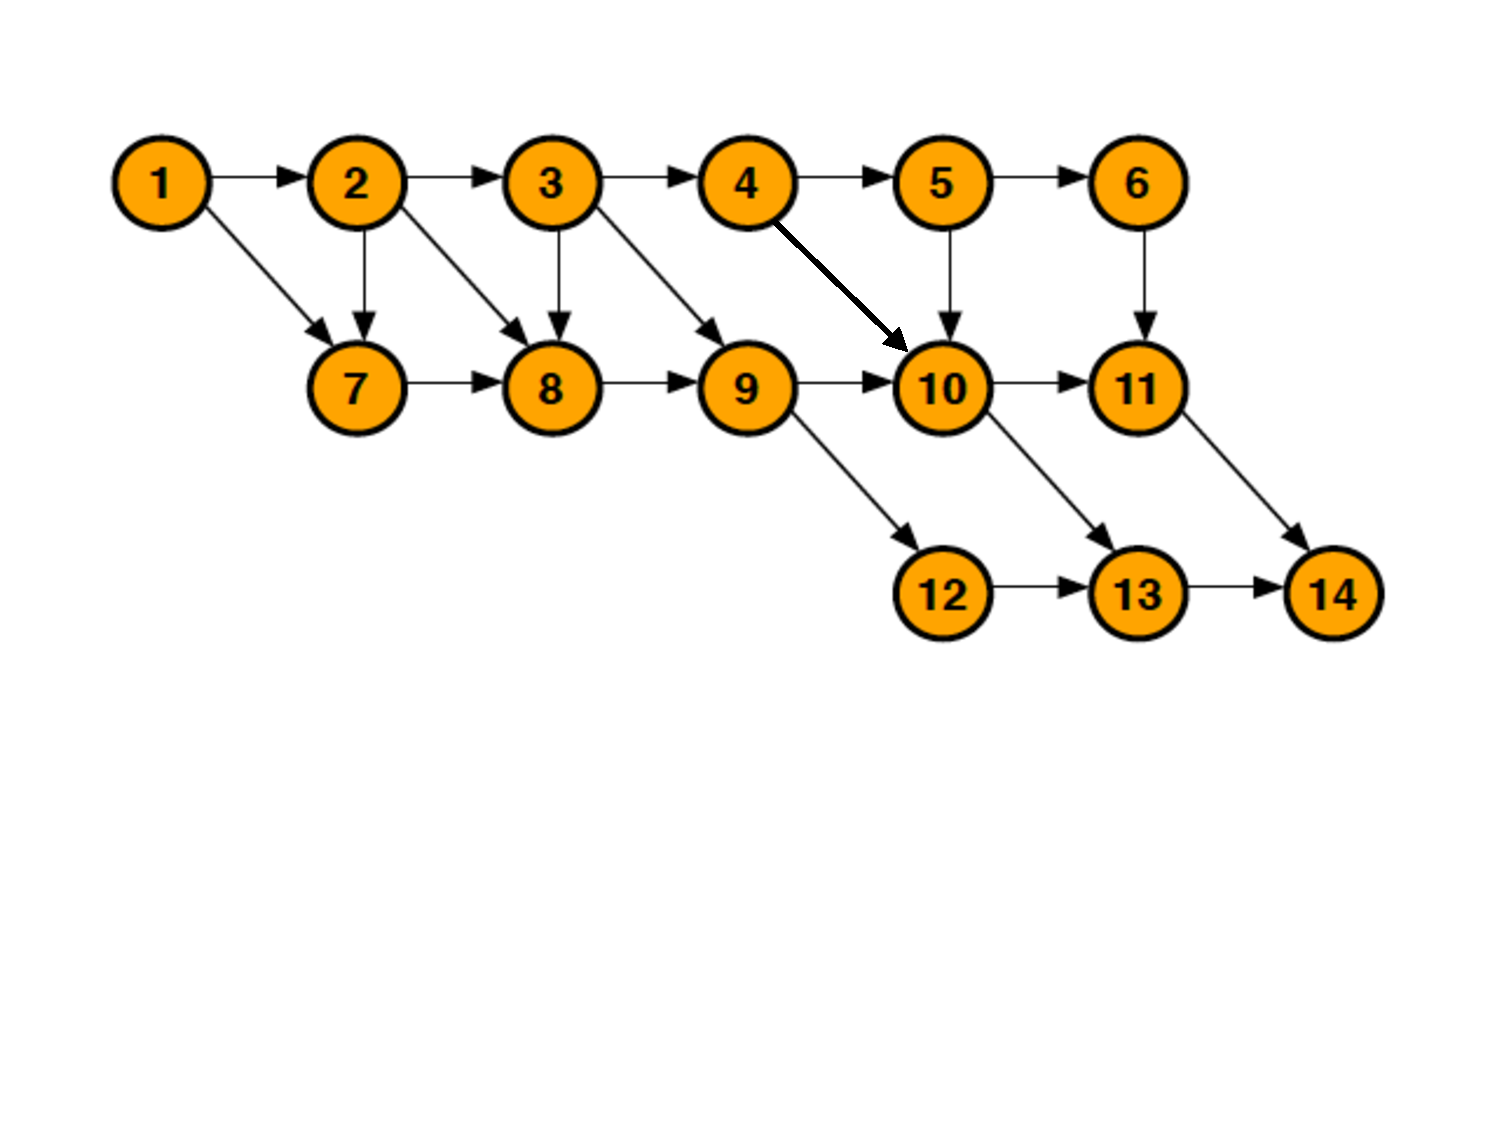
\includegraphics[scale=0.45]{dag_ps9.pdf} 
        \end{center}
        \end{figure}
        % ----------
    
        \begin{solution}

        \end{solution}


\end{enumerate}


\end{document}


